\section{Was sind Visualisierungs Applikationen [FK]}\label{sec:visualization}
Visualisierungs Applikationen sind eine Möglichkeit Daten als Grafiken widerzuspiegeln. Die Daten können auf vielfältige Art und Weise zusammengestellt werden. Nicht jede Visualisierungs Applikation kann dieselben Datenquellen benutzen und verarbeiten. In Microsoft Word kann man zum Beispiel ausschließlich Microsoft Excel Tabellen für die Diagramme einfügen. In Spezialisierteren Applikationen können weitaus mehr Datenquellen verwendet werden wie Daten direkt aus einer Datenbank auslesen oder mit einer REST [\ref{sec:REST}] Schnittstelle von einem Server zu bekommen.
\subsection{Warum Visualisierungstools}
Viele Unternehmen sammeln täglich riesige Mengen an Daten über ihre Kunden, Mitarbeiter, den Markt und viele andere Dinge, aber dieses Wissen ist einzeln betrachtet in bedeutungslosen Zahlen versteckt.
"Die Datenvisualisierung ermöglicht es, sich bei der Auswertung und Präsentation von Daten auf das Wesentliche zu konzentrieren. Die Entscheidungsfindung lässt sich dadurch erleichtern. Während die Auswertung von Daten, die in reiner Tabellenform vorliegen, aufwendig und zeitraubend ist, sind mit der Datenvisualisierung enorme Zeiteinsparungen realisierbar. Oft ist auf den ersten Blick erkennbar, welche Informationen und Zusammenhänge die Daten bereithalten." (\cite{vorteileDV})
Diese Diagramme können helfen, Marktveränderungen vorherzusagen oder den Gewinn durch intelligente Kostenreduzierung zu erhöhen. 
Dies könnte entweder von einem Betreiber genutzt werden, der ansprechende Diagramme für seine Präsentationen und Berichte verwendet, oder von Datenanalysten, die diese Diagramme studieren und nützliche Informationen ableiten, um Fragen zu beantworten wie "Warum steigt der Markt in Großbritannien, obwohl es den Brexit gibt, und wie können wir das, was in dieser Region funktioniert, in andere Regionen bringen?

\subsection{Visualisierungen in Softwareprodukten}
Nicht nur Marktorientierte Betriebe müssen einen Überblick über ihre Produkte haben, sondern auch Softwareunternehmen oder deren Kunden. Visualisierung kann nämlich auch dazu verwendet werden um Softwareprodukte zu Kontrollieren. Jedes Vernünftige Softwareprodukt gibt eine Menge an Informationen in Form von Log Dateien ab. Der Inhalt von Log Dateien kann alles Mögliche sein von harmlosen Statusmeldungen bis hin zu etwaigen schweren Problemen in Form von Fehlercodes. Fehlercodes wiederum können ebenfalls gänzlich unterschiedlich sein. Ob es ein Problem mit der Hardware gibt das zum Beispiel der Speicher voll ist oder das Netzwerk überlastet ist, Ein Benutzer eine falsche Eingabe ausgeführt hat welche nicht im Programm überprüft wurde oder gar ein Programmfehler der zu einem Absturz geführt hat. Egal welches Problem es ist, man sollte darüber informiert werden und wenn Probleme häufiger auftreten muss man sich darum kümmern. Natürlich gibt es Lösungen die Log Files Manuell auszulesen und den Fehler zu beheben aber es können Probleme öfters vorkommen was nicht sofort auffällt. Was zu dem Punkt führt das es viel einfacher wäre, wenn jeder auf einem Blick sieht wie stark das Netzwerk belastet ist oder wie viele Abfragen es auf einen Server gibt. An dieser Stelle kommen Visualisierungsapplikationen ins Spiel.
\begin{figure}[H]
    \centering
    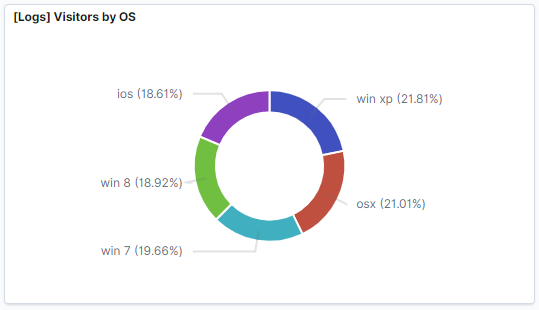
\includegraphics[scale=1.3]{images/sampleLogs1.PNG}
    \caption{Besucher pro Betriebssystem aus Log Dateien}
\end{figure}
\begin{figure}[H]
    \flushleft
    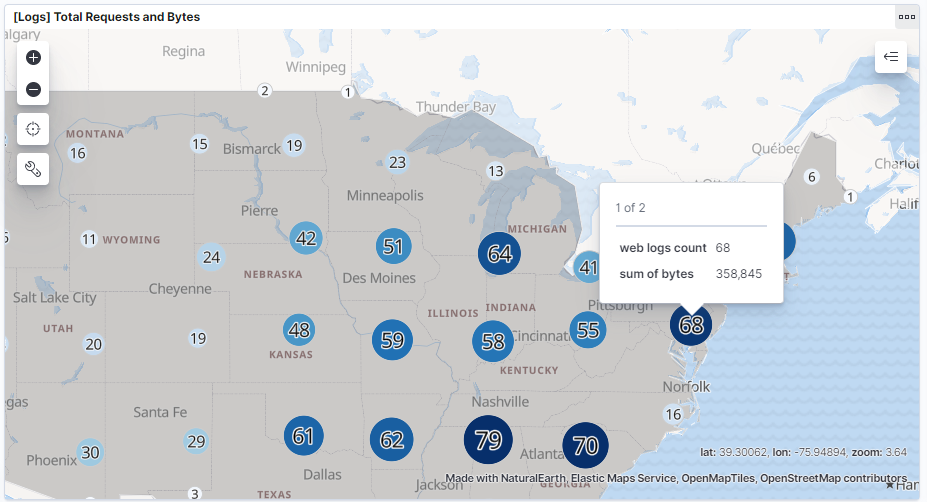
\includegraphics[scale=0.85]{images/sampleLogs2.PNG}
    \caption{Netzwerkverkehr pro amerikanischen Bundesstaat}
\end{figure}
Anhand dieser zwei Beispiele sieht man sehr schön wie nützlich es sein kann seine Daten Live anzusehen. Auf einem Blick sieht man wie hoch die Auslastung in den einzelnen Bundestaaten ist. Somit kann man Maßnahmen ergreifen und zum Beispiel die Serverkapazitäten in den Östlichen Bundesstaaten erhöhen und in den Westlichen verringern, weil dort viel Seltener Anfragen an die Server gestellt werden. Durch gezielteres Lösen von Problemen kann so einiges an Kosten gespart werden. Ein weiterer Großer Vorteil von diesen Visualisierungen ist das Nicht-Techniker die Möglichkeit bekommen auf schnellten Wege an die benötigten Informationen zu kommen und in Meetings einzusetzen. Die Reaktion auf Softwareprobleme kann somit um einiges beschleunigt werden. 